\documentclass[12pt,a4paper]{report}
\usepackage{tikz}
\usepackage{hyperref}
\usepackage{amsmath}
\usepackage{amssymb}
\usepackage{amsthm}
\usetikzlibrary{arrows,positioning}
\tikzset{ >=stealth', punkt/.style={ rectangle, rounded corners, draw=black, very thick, text width=6.5em,minimum height=2em, text centered}, pil/.style={ ->, thick, shorten <=2pt, shorten >=2pt,}}
\begin{document}
 \href{doc/phil/PhilProblems.html}{Previous} 
 \href{doc/phil.html}{Up} 

 \href{doc/phil/PhilSituations.pdf}{PDF} 
\title{Phil Situations}

\tableofcontents

\part{doc/phil/PhilSituations/BeeWaggle.html|Bee Waggle}
When a foraging bee discovers a supply of food, it returns to the hive and does
a waggle dance. The rest of the hive then flies out in a certain direction and
distance to locate the food. In some sense, the bee communicates the information
of the food supply to the hive.

Can't we explain why a particular bee on one
occasion does that by invoking the pattern that
it's an instance of? What would it mean to say of
a bee returning from a food source that it's
turnings and wiggling has occurred \emph{because}
they're part of a complete dance? This is related
to distinction of pattern governed vs rule
obeying behavior. (cite some reflections on
language games) Ruth milliken, Sellars student,
devotes her career to this, developing the field
of teleosemantics and writing about it in
Language, Thought, and Other Biological
Categories.

A simpler example than the bee one for this is
that beavers slap their tail when there's danger
and beavers flee when they hear another beaver
slap its tail.

The idea of teleosemantics is an evolutionary
sort of semantics. Acknowledge language use is
normative (make distinction between correct and
incorrect use). You have to draw the distinction
in the way that's compatible with any degree of
badness of the participants actually following
the rules. We look at a reproductive family, the
normal explanation (a tehcnial term) of tail
slapping is that, in the evolutionary history,
lives were saved by it. When the explanation of
the persistence of tail slapping turns on
particular eventsi n the past where things worked
well that way (expressed in terms of
counterfactuals - no tail slap, then species dies
out), then we can say its part of the proper
function (technical term) to perform that
behavior. This  solves some puzzle cases: it
allows us to say the proper function of sperm is
to fertilize eggs even if a vanishingly small
fraction of them actually do (because if they
hadn't fertilized eggs in the past, there
wouldn't be sperm now).

Well, this is the form of explanation for semantics, not a beaver tail slaps
that aren't involved in more complicated interactions than that. Because the
same thing can happen when the reproductive families are uses of words. Where
you can explain why, you know, we use the word Aristotle, as we do, if has
having a proper function of, in the end, referring to Aristotle, because if
people in the past had not used it, in particular ways, we wouldn't be using
it today. And similarly, for predicates, and so on. She says, These are not
biological norms. But we can understand words as having proper functions in the
same sense in which even in the merely biological case, we can understand things
as having proper functions. And we can understand them as having proper
signaling functions. So there's a proper function for producing these things
and a proper function for receiving them. There, the analogy of the of the tail
slaps is a good one.

But in order to get semantic cut to understand semantic content, we don't need
to use any principles of explanation that aren't already intelligible


\part{doc/phil/PhilSituations/ChildrensGame.html|Childrens Game}

A mother lets me watch her kids and says to me: Show the children a game. When she returns, she sees me teaching them to gamble with
dice. She angrily exclaims I didn't mean that sort of game! Must the exclusion
of the game with dice have come before his mind when he gave me the order?

It's true that she did mean not that sort of game. but she need not have had the conscious thought at the time of the request. Somehow her request made a normative division of proper responses.

If you find this puzzling that, nonetheless, what you did was an inappropriate response to her request, then you are trapped in a possibly Cartesian trap. You're missing what distinguishes a sign from a piece of wood.

From: \cite{wittgenstein2010philosophical}

Frac $\frac{a}{b}$!

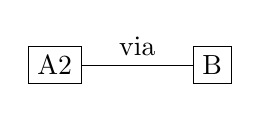
\begin{tikzpicture}
  \path (0,0) node[draw] (A) {A2};
  \path (2,0) node[draw] (B) {B};
  \draw (A) -- (B) node[midway,above = 0 em] {via};
\end{tikzpicture}


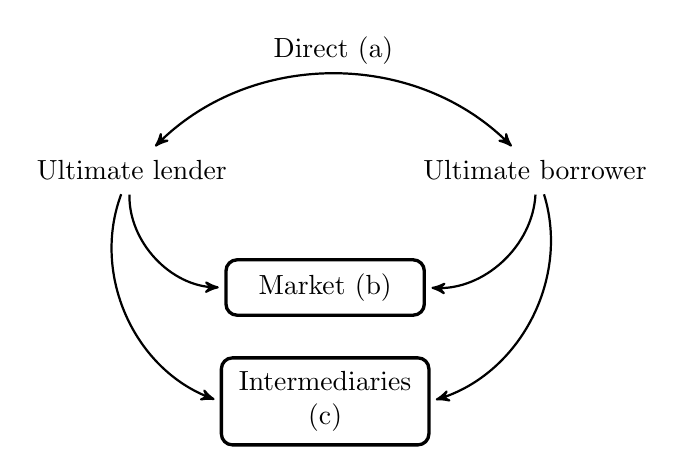
\begin{tikzpicture}[node distance=1cm, auto,]
    %nodes
    \node[punkt] (market) {Market (b)};
    \node[punkt, inner sep=5pt,below=0.5cm of market]
    (formidler) {Intermediaries (c)};
    % We make a dummy figure to make everything look nice.
    \node[above=of market] (dummy) {};
    \node[right=of dummy] (t) {Ultimate borrower}
      edge[pil,bend left=45] (market.east) % edges are used to connect two nodes
      edge[pil, bend left=45] (formidler.east); % .east since we want
                                                % consistent style
    \node[left=of dummy] (g) {Ultimate lender}
      edge[pil, bend right=45] (market.west)
      edge[pil, bend right=45] (formidler.west)
      edge[pil,<->, bend left=45] node[auto] {Direct (a)} (t);
   \end{tikzpicture}

   \vspace{1em}
   \emph{Inspired by figure 1.1 in ``Financial Markets and Institutions'' 5E
     by Howells and Bain.}



\part{doc/phil/PhilSituations/ClassicalBehaviorism.html|Classical Behaviorism}
This is related to the problem of: suppose you follow a rule. You use a
representation of that rule to train the next generation to follow the rule.
How do we know that the same rule is being passed on? Isn't it like a game of
telephone, given the ambiguity of following rules (gerrymandering problem - you
have a rule in your head and punish me for lifting the glass of water, but I
interpret this as punishment for lifting my arm or one of a million other
possible explanations). Brandom's response:

Well, maybe so and maybe it a given rule isn't as stable as we think. I mean,
it's only if it had enough coherence and enough stability, that we're here.
(Anthropomorphic principle). And when Wittgenstein harps on this, you know, unless
as a matter of fact, we tended to go on the same way when trained the same way,
to a remarkable extent, we wouldn't get a language game off the ground.

I should mention that this gerrymandering issue is what was wrong with classical behaviorism from an empirical point of
view. \footnote{What was wrong with
classical behaviorism, from a \emph{conceptual} point of view, is we can see it with
the wisdom of hindsight is just a larval stage on the way to functionalism. As
all of the considerations that lead people to think have direct stimulus
response connections, are satisfied still, if you allow intervening states. It's still an empirical undertaking, and so on. But there's a
lot more formal power, you can get Turing machines, if you can get functional
states, so you can get a lot farther. That's why
nobody should be a classical behaviorist anymore: be a functionalist, you get
all the advantages, and a lot more expressive power.} Remember, the stimulus and response were supposed to be
objective features of the critters you were looking at. So that the behavioral
scientist modeled on the natural scientist, her own conceptual scheme was not
supposed to be involved in characterizing the behavior of these critters. But
if you ask sort of classical studies, so I take the rat, and set him down four
steps away from the bar, and train him, then if he walks four steps forward and
presses down on the bar, he'll get a rat yummy. And that stimulus, let's say,
the light goes on, walks, four steps, pushes down on the bar gets a rat yummy.
We indoctrinate him with that, conditioned learning, he can do that. And now
we ask the behavioral scientist. And now if I put in eight steps away from
the bar, what do you predict he's going to do? Is he going to go four steps
forward and move his paw up and down? Is that the behavior that has been
associated with the stimulus? Or would you predict that he'll go eight steps
forward and press down on the bar. That is, the right description is that he'll
go from where he is to the bar and press on the bar? Well, the minute you think
about this, you realize that we can gerrymander, what he was taught,
there are many descriptions, that that are available to us for what he was
taught. And in fact, no one who works with the animals would expect him to
move four steps forward, and not be pressing on the bar. But why
is that? Is that something that you without importing any understanding of
this are objectively reading off of the situation? Or have you, in fact, all
along been importing, your characterization of what the regularity
is that you are, that you're characterizing? This is actually empirical as well a methodological
problem. What is the prediction that you're supposed to make at this point?
And how do you justify the one rather than rather than the other by your
methodological lights?

\part{doc/phil/PhilSituations/MontaigneDog.html|Montaigne Dog}
Montaigne is impressed that his dog, when chasing
a rabbit and coming to a fork, runs a little way
down one of the paths and smells no rabbit, then
immediately runs down the other fork of the path
without stopping to smell to check if the rabbit
went that way. (CITE?)

The dog is acting in accordance with the
disjunctive syllogism. Do we say that the dog
understands disjunction?
\part{doc/phil/PhilSituations/ToothPain.html|Tooth Pain}
Imagine a community that talked about having gold or silver in one’s teeth,
and extends that practice to talk about having pain in one’s teeth. If, as a
matter of contingent fact, the practitioners can learn to use the expression
‘in’ in the new way, building on (but adapting) the old, they will have
fundamentally changed the \emph{meaning} of ``in". This can be seen by the
fact that, in the old practice, it made sense to ask where the gold was before
it was in one’s tooth, whereas in the new practice asking where the pain was
before it was in the tooth can lead only to a distinctively philosophical kind
of puzzlement.

\cite{brandom2019some}

\bibliography{my}
\bibliographystyle{amsalpha}
\end{document}